% Created 2021-04-21 Wed 13:13
% Intended LaTeX compiler: pdflatex
\documentclass[11pt]{article}
\usepackage[utf8]{inputenc}
\usepackage[T1]{fontenc}
\usepackage{graphicx}
\usepackage{grffile}
\usepackage{longtable}
\usepackage{wrapfig}
\usepackage{rotating}
\usepackage[normalem]{ulem}
\usepackage{amsmath}
\usepackage{textcomp}
\usepackage{amssymb}
\usepackage{capt-of}
\usepackage{hyperref}
\author{190022658}
\date{\today}
\title{W11-SP Report}
\hypersetup{
 pdfauthor={190022658},
 pdftitle={W11-SP Report},
 pdfkeywords={},
 pdfsubject={},
 pdfcreator={Emacs 27.2 (Org mode 9.5)}, 
 pdflang={English}}
\begin{document}

\maketitle

\section{Overview}
\label{sec:org9e5d6f6}
\begin{itemize}
\item The objective of this practical was to gain experience with processes and simple Inter-process Communication (IPC) in C.\\
\item This objective was to write a program that creates multiple processes in C, and uses pipes for inter-process communication.\\
\end{itemize}


\section{Design}
\label{sec:org153d255}
In order of implementation -\\
\subsection{Pipeline}
\label{sec:orgff6e5da}
\begin{description}
\item[{Pipeline.h}] We had to implement a Pipeline struct for use in Pipeline.c. This is to store the ``user-defined'' functions.\\
The Pipeline stuct has two variables for good use\\
\begin{itemize}
\item funcs (Function*)\\
\item funcsSize (int)\\
\end{itemize}

\item[{Pipeline.c}] Implentation of all the functions for the pipeline.\\
\begin{description}
\item[{new\_Pipeline}] This uses malloc to create the \texttt{Pipeline} structure, assign 0 to funcsSize (as there are no functions in the array yet), and to create the \texttt{Function} array. This returns a pointer to the pipeline structure created.\\
\item[{Pipeline\_add}] This reallocates space in the \texttt{Function} array to add more functions. If there is no more space available, the function returns false and the program that the user defined exits. Otherwise, the function is added to the pipeline and the size of array is incremented.\\
\item[{Pipeline\_execute}] This function runs all of the functions in the array (which is inside the Pipeline structure), in different processes. There were two ways of doing this, one is to create multiple process for a single parent and giving them a ``function to do''. This makes quite a lot of sense conceptually, so I implemented this (Pipeline\_execute\_alt) along with what the specifications said. The specifications said to create a child for every parent.\\

In the specification's one implementation I used a prevFd[2] variable to keep track of the last pipe used. This is to be used as input for the process in the current iteration. After that there is a loop that creates a pipe (to be used as output for the function). There is a fork function then and the child pid value is stored inside a variable called child. After that the program checks for an error and responds accordingly. Then for the parent, we close the pipes not needed (although what happens to the ones already opened, do they need to be closed? The alt method contains another way to handle pipes). After closing the pipes, the function of current index in the pipeline object is executed with the prevFd[0] being input and fd[1] being output. After that the parent waits for its child and exits without error. Note that it does not exit if it is the parent of all the other functions. It would still work but the cleanup function will not be called. Lastly the prevFd is assigned as fd.\\

This loops on till all the functions are executed. The last process created is not needed since the parent does its job. So it is exited using an if statement. The program somehow works without it. The other way is to ``int child = i == N-1 ? 1 : fork();''. This way the process is never created and the current process becomes the ``father'' (according to the if statement).\\
\end{description}
\end{description}

\subsection{TestPipeline}
\label{sec:org5d6cb9a}
This is described in the Testing section.\\


\section{Testing}
\label{sec:org7eebaae}

This program works as showed in the requirements.\\

\begin{verbatim}
❯ make
clang -g -Wall -Wextra -c Pipeline.c
clang -g -Wall -Wextra SumSquaresPipeline.o Pipeline.o -o SumSquaresPipeline
clang -g -Wall -Wextra SievePipeline.o Pipeline.o -o SievePipeline

❯ ./SievePipeline < sieve1.in
Setting up pipeline to sieve out the first 5 prime numbers up to 15
generateInts: process 378264, parent 342925
sieveInts: process 378265, parent 378264: prime = 2
sieveInts: process 378266, parent 378265: prime = 3
sieveInts: process 378267, parent 378266: prime = 5
sieveInts: process 378268, parent 378267: prime = 7
sieveInts: process 378269, parent 378268: prime = 11

❯ ./SumSquaresPipeline < squares.in
Setting up pipeline to calculate the sum of squares of integers 1 to 10.
generateInts: process 378320, parent 342925
squareInts: process 378321, parent 378320
sumIntsAndPrint: process 378322, parent 378321
sumIntsAndPrint: result = 385
\end{verbatim}

Along with that, I used a copy of TestStack.c (RPN calculator practical) as TestPipeline.c, there are multiple functions that are used to test the Pipeline implementation. They are self-explanatory and they all pass. The third test uses the pipeline implementation to double and print the result (idea from specification).\\

\begin{verbatim}
This should double the number using a pipeline
Enter a number: 3
Received int: 6
Is that the expected output (y/n): y

Pipeline Tests complete: 3 / 3 tests successful.
----------------
\end{verbatim}

\begin{figure}[htbp]
\centering
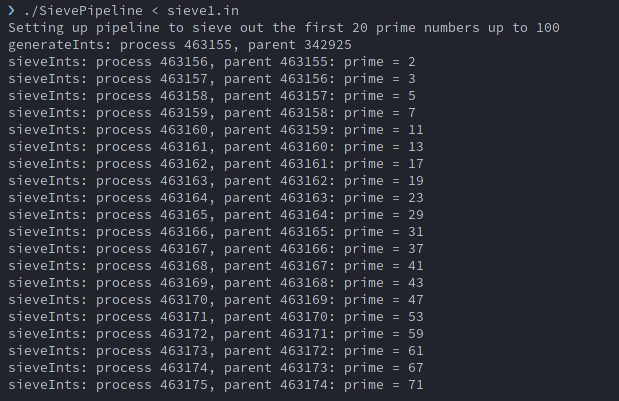
\includegraphics[width=.9\linewidth]{./images/sieveInts.png}
\caption{\label{Sieve Ints}Image showing that code works with a big number}
\end{figure}

\section{Conclusion}
\label{sec:orgd3f3b36}
This practical was quite helpful in understanding how pipes and processes work. This was quite new to me, and understanding the system processes was very interesting too.\\
\end{document}
